\documentclass[11pt]{article}
\usepackage[margin=1in]{geometry}
\usepackage{amsmath,amssymb,booktabs,graphicx,hyperref,microtype}
\usepackage{enumitem}
\usepackage{pgfplots}
\pgfplotsset{compat=1.16}
\usepackage[backend=biber,style=numeric,sorting=none]{biblatex}
\addbibresource{references.bib}
\title{When Does Language-Model Reasoning Help Variational Quantum Circuit Search?\\
From Capacity-Controlled Benchmarks to Semantic Quantum Autoencoders}
\author{Anonymous authors}
\date{\today}

\begin{document}
\maketitle

\begin{abstract}
Large language models (LLMs) are increasingly used as agents that propose variational quantum circuit (VQC) architectures, but it is unclear when language-model reasoning provides an advantage over ordinary search.
We first summarize capacity-controlled VQC benchmarks in which Random, Evolutionary, and Greedy search became practically equivalent after circuit size, training, and evaluation budgets were matched.
This negative result suggests that an LLM cannot exploit much of its domain knowledge when the search problem is reduced to a flat gate grammar.
We therefore introduce a semantic quantum-autoencoder (QAE) benchmark in which the proposer receives an explicit Hamiltonian, a latent/trash-qubit assignment, and a fixed resource budget.
The task compresses four-qubit open-chain transverse-field Ising ground states to two latent qubits.
Every candidate is an ordered sequence of exactly sixteen gates --- twelve trainable single-qubit rotations (free axis and qubit) and four CNOTs (free wiring), with completely free gate ordering; only the architecture proposer differs.
We compare four conceptually organized methods --- Random (no semantics, breadth-only), Greedy (no semantics, validation-guided local refinement), LLM-Open (semantics, open-loop batch), and LLM-Closed (semantics, adaptive closed-loop) --- each with eight candidate evaluations per seed and a version-pinned API model (\texttt{gpt-5.4-mini-2026-03-17}).
A first, single-start experiment (v3) found a large semantic advantage but also that its single-start adaptive arms struggled: Greedy landed significantly below Random and no closed-loop benefit over open-loop was detected.
A pre-registered multi-start follow-up (v4; four warm starts, then four refinement evaluations) confirms that diagnosis.
On the held-out test trash fidelity $F_{\rm trash}=\langle 00|\rho_{\rm trash}|00\rangle$, LLM-Open reaches $0.9643$ versus $0.8677$ for Random (paired gain $+0.0965$, 95\% CI $[0.082, 0.112]$, $d_z=3.5$, 12/12 seeds, exact Wilcoxon $p=0.00049$), replicating the v3 pool ($0.9653$) with an independently drawn pool; Greedy recovers to Random-parity with a genuine refinement gain ($+0.0635$, 10/12 seeds); LLM-Closed's duplicate proposals largely disappear, yet no additional closed-loop benefit over the open-loop batch is detected ($-0.0085$, $p=0.13$).
The result is exploratory rather than a general LLM-superiority claim: it is a small noiseless four-qubit simulation with a single pinned model.
The main conclusion is conditional: language-model reasoning becomes useful when the task exposes semantic structure that can be converted into circuit priors, rather than merely asking the model to sample gate syntax.
\end{abstract}

\section{Introduction}

Variational quantum algorithms depend on parameterized quantum circuits whose architecture determines expressivity, trainability, hardware cost, and the correlations that can be represented.
Circuit design is therefore a joint discrete--continuous problem: a discrete architecture is chosen first, while continuous angles are optimized by a numerical training loop.
Previous work has characterized circuit expressibility and entangling capability \cite{sim2019}, developed quantum architecture search (QAS) algorithms \cite{du2022}, and recently used language-model agents to propose and refine VQCs \cite{knipfer2026}.

The motivation for an LLM searcher is different from the motivation for a generic black-box optimizer.
A language model can read a natural-language task description, identify physical or structural priors, and translate them into architectural hypotheses.
However, that advantage disappears if the experimental interface hides the task semantics and exposes only a small list of allowed gates.
This distinction is central to the present work.

Our study proceeds in two stages.
First, we use the project's prior capacity-controlled benchmarks as a diagnostic.
When candidate circuits were matched in trainable capacity and all searchers received the same validation feedback, Random, Evolutionary, and Greedy search were practically equivalent on the synthetic T1 task.
The task still benefited from selecting the best of several candidates, but no sophisticated search strategy was required.
Second, we design a QAE task whose structure is directly meaningful to an LLM.
The proposer is told which qubits must become ``trash'', which qubits form the latent representation, the Hamiltonian interaction graph, and the fact that the target ground states can be represented with real amplitudes.

Our research question is therefore not ``Does an LLM always beat random search?'' but:
\begin{quote}
\emph{When does task-aware language-model reasoning improve VQC architecture search under exact capacity control?}
\end{quote}

\section{Related Work}

\paragraph{VQC architecture quality.}
Sim et al.\ proposed operational measures of expressibility and entangling capability and emphasized that useful circuit design must also account for depth, two-qubit gates, connectivity, and parameter count \cite{sim2019}.
Du et al.\ formulated quantum circuit architecture search as an automated VQA design problem \cite{du2022}.
More recent embedding-aware QAS work argues that data embedding and circuit structure should not be optimized independently \cite{dai2026}.

\paragraph{LLM agents for VQC design.}
Knipfer et al.\ introduced an agentic loop in which an LLM proposes PennyLane VQCs, receives training and validation feedback, and iteratively changes the architecture \cite{knipfer2026}.
Their experiments show that language models can discover interpretable motifs such as star entanglement and data/computation-qubit specialization, while also exhibiting invalid-code and exploration-collapse failure modes.
These results motivate a controlled test that separates architecture reasoning from parameter optimization.

\paragraph{Quantum autoencoders.}
Romero, Olson, and Aspuru-Guzik introduced QAEs as trainable circuits that compress families of quantum states into a smaller latent subsystem while mapping discarded qubits to a reference state \cite{romero2017}.
They demonstrated the idea on ground-state families from quantum simulation.
Recent work has applied QAEs to anomaly detection \cite{frehner2025,elalami2025}, while Agha et al.\ explicitly use a genetic algorithm to search QAE architectures \cite{agha2025}.
This makes QAE a natural benchmark for comparing a language-model proposer to standard architecture-search baselines.

\section{Lessons from the Earlier Controlled Benchmarks}

The earlier project stages were designed to remove confounders that can make an LLM look better or worse for the wrong reason.
All candidate circuits were matched in parameter capacity, every search method used the same trainer and data split, the candidate budget was identical, and protected-test metrics were quarantined from the search loop.

On capacity-controlled T1-v2, the protected-test RMSE medians were $0.01775$ (Random), $0.01715$ (Evolutionary), and $0.01689$ (Greedy).
A pre-specified paired equivalence test concluded that all three pairs were practically equivalent within $\delta=0.002$.
At the same time, selecting the best of $B=25$ validation candidates improved performance relative to a fixed circuit.
Thus architecture selection mattered, but the specific search algorithm did not.

Two broader lessons followed.
First, a simple benchmark can be dominated by task-specific analytical estimators, so success on a learned model does not imply a useful quantum or search advantage.
Second, the HIGGS follow-up showed that data scarcity, a mis-tuned inherited learning rate, and PCA information loss could push the VQC into a degenerate regime in which architectural effects were obscured.
After correcting those factors, the signs of the trainable-vs-frozen and entangled-vs-product comparisons changed.
We therefore treat \emph{task qualification} as a prerequisite for judging a search algorithm.

These findings motivate a new benchmark in which the proposer receives a decision that is both controlled and semantically meaningful.

\section{Semantic Quantum-Autoencoder Benchmark}

\subsection{Task}

We use the four-qubit open-chain transverse-field Ising Hamiltonian
\begin{equation}
H(h) = -\sum_{i=0}^{2} Z_i Z_{i+1} - h\sum_{i=0}^{3} X_i,\qquad h\in[0.2,2.0].
\end{equation}
For each value of $h$, the exact ground state $\lvert\psi(h)\rangle$ is obtained by diagonalizing the $16\times16$ Hamiltonian.

The QAE encoder $U_\theta$ acts on all four qubits.
Qubits $q_0,q_1$ are the latent subsystem and $q_2,q_3$ are the trash subsystem.
The training objective is to make the trash qubits independent of the input and equal to the reference state $\lvert 00\rangle$.
We therefore maximize
\begin{equation}
F_{\rm trash}(\theta)
=
\frac{1}{N}\sum_{j=1}^{N}
\Pr_{\theta,\psi(h_j)}(q_2q_3=00),
\end{equation}
or equivalently minimize $1-F_{\rm trash}$.
Writing $\rho_{\rm trash}$ for the reduced density matrix of $q_2,q_3$ after the encoder, this is the trash-state fidelity $F_{\rm trash}=\langle 00|\rho_{\rm trash}|00\rangle$: if $F_{\rm trash}=1$ the trash subsystem is exactly $\lvert00\rangle$ and the input-dependent information has been routed into the latent subsystem.
$F_{\rm trash}$ is a compression-side trash/reference fidelity; it is not automatically identical to an end-to-end reconstruction fidelity.
Throughout, ``held-out (protected) test'' refers only to the data split --- the 64 unseen $h$ values never used for training, architecture selection, or any feedback --- while the fidelity formula itself is identical on every split.
For a perfect encoder, the input family is compressed into the two latent qubits and the trash state is always $\lvert00\rangle$.

This is the same basic compression principle as the original QAE: successful compression corresponds to disentangling the discarded subsystem and mapping it to a fixed reference state \cite{romero2017}.

\subsection{Exact capacity control in a neutral space}

Every candidate is an \emph{ordered sequence of exactly sixteen gates}:
\begin{itemize}[nosep]
\item four qubits ($q_0,q_1$ latent; $q_2,q_3$ trash);
\item allowed gates: RX, RY, RZ, CNOT only;
\item exactly twelve trainable single-qubit rotations, each with free axis (no per-axis quota) and free target qubit;
\item exactly four CNOTs, each with free control and (different) target; the same directed pair may repeat at different positions;
\item gate ordering completely free.
\end{itemize}

Twelve rotations correspond to three trainable local rotations per qubit and four CNOTs to roughly one two-qubit entangler per qubit; this is a benchmark capacity choice, not a claim that the ratio is physically optimal.
An earlier pilot (v1/v2) constrained candidates to a rigid rotation-layer/CNOT-layer layout; the primary v3 experiment drops that layout because it was a convenience of the pilot, not a technical necessity.
Capacity is verified programmatically for every candidate of every method.
The numerical optimizer, number of epochs, parameter initialization distribution, data splits, and validation-selection rule are shared by all methods.
The LLM never chooses continuous parameter values.
The full protocol, including the analysis plan, was committed before the experiment ran and amended once --- also before any protected-test inspection --- to extend the bounded JSON-repair policy to capacity-invalid pool entries.

Each candidate is optimized with Adam for 60 epochs at learning rate $0.05$.
The checkpoint with the best validation trash loss is selected.
For each of twelve verification seeds, 32 fresh $h$ values are sampled for training, 12 for validation, and a fixed unseen 64-point grid is used only for protected-test evaluation after selection.
Each architecture-search method receives exactly $B=8$ candidate evaluations.

\subsection{Search methods: a conceptual organization over semantics and search policy}

The four primary methods organize two ingredients --- \emph{task semantics} in the proposal distribution and \emph{validation-guided adaptivity} during search --- while sharing capacity, trainer, data, and budget:

\begin{center}
\begin{tabular}{ll}
\toprule
Random & no semantics; breadth-only (8 independent draws)\\
Greedy & no semantics; multi-start + validation-guided local refinement\\
LLM-Open & semantics; open-loop diverse proposal batch\\
LLM-Closed & semantics; multi-start + validation-guided adaptive refinement\\
\bottomrule
\end{tabular}
\end{center}

We deliberately do not present this as a causal $2\times2$ factorial: Random and Greedy differ in allocation policy as well as feedback, and LLM-Open versus LLM-Closed compares open-loop batch search against adaptive closed-loop search rather than isolating ``the pure effect of feedback.''

Two allocation designs were run in sequence.
The first experiment (\textbf{v3}) used single-start adaptive arms: Greedy was one random start plus seven local mutations, and LLM-Closed proposed all eight candidates sequentially.
After inspecting v3 --- which is preserved unchanged as a diagnostic --- we pre-registered a multi-start follow-up (\textbf{v4}, protocol committed before the v4 matrix ran) in which each adaptive arm spends its budget as \emph{four warm-start evaluations followed by four refinement evaluations}.
The v4 definitions follow; v3's differences are noted inline.

\paragraph{Random.}
Eight architectures sampled independently and uniformly from the neutral space: uniform axis and qubit for each rotation, uniform directed pair (with replacement) for each CNOT, uniform interleaving of the sixteen gates.
(v4 draws fresh streams; it is an independent replication, not a replay of v3.)

\paragraph{Greedy (v4: 4+4).}
Phase 1: four independent Random draws are trained and evaluated; the best by validation loss becomes the incumbent.
Phase 2: four further evaluations, each applying exactly one structural change to the incumbent, chosen uniformly among: change one rotation's axis, change one rotation's qubit, change one CNOT's control, change one CNOT's target, or swap two gate positions; the mutation is accepted only if its validation loss improves on the incumbent's.
Every evaluated mutation consumes budget whether accepted or not.
(v3: one random start plus seven mutations.)

\paragraph{LLM-Open (version-pinned API).}
One chat-completion call to \texttt{gpt-5.4-mini-2026-03-17} (temperature $0.7$) sends the physics/task card of Appendix~\ref{app:prompt} --- Hamiltonian, real-ground-state property, nearest-neighbour interaction structure, latent/trash roles, and the exact resource contract --- and requests eight distinct candidates in a structured JSON gate-list schema.
The v4 pool returned eight valid, distinct architectures in a single call (the v3 pool needed one bounded capacity-repair call, per its pre-registered amendment).
No validation result is ever shown to this arm.

\paragraph{LLM-Closed (v4: 4+4).}
Same pinned model, same task card.
Phase 1: one batch call per seed requests four distinct candidates \emph{without} any validation feedback, with an explicit instruction to aim for structural diversity; all four are trained and evaluated.
Phase 2: four sequential calls; each prompt appends the validation trash fidelities and duplicate flags of all candidates evaluated so far in that seed --- never held-out test values --- and requests one new candidate.
Invalid or duplicate proposals consume one of the eight evaluations and are replaced by flagged random circuits, so budget accounting is identical to every other method.
(v3: all eight proposals sequential from the start.)

Both LLM arms allow up to two JSON-repair retries per call; every attempt is recorded (system prompt, user prompt, raw response, token counts, latency, model snapshot).
All API usage runs under a hard \$2.00 cumulative cost cap enforced before every call; the v4 benchmark used 66 calls and 48{,}952 input + 19{,}177 output tokens (v3: 98 calls, 99{,}758 + 18{,}342).

\paragraph{Historical baselines (v2).}
An earlier verification in the rigid-layout space compared the LLM pool against an RY-only random control, an equal-budget evolutionary searcher, and a hand-designed reference encoder; the LLM pool beat all of them (mean $0.9700$ vs.\ $0.9424$, $0.9005$, $0.8889$; all $p\le0.0015$).
Those results (\texttt{outputs/qae\_tfim\_api\_v2/}) are retained as context; v4 is the primary experiment.

\section{Results}

\subsection{v3: the single-start diagnostic}

The v3 experiment (single-start adaptive arms) found means of $0.9653$ (LLM-Open), $0.9553$ (LLM-Closed), $0.8721$ (Random), and $0.7667$ (Greedy) on the held-out test trash fidelity.
Three observations motivated the v4 follow-up.
First, Greedy landed significantly \emph{below} Random ($-0.1055$, 2/12 wins, $p=0.005$) despite functioning correctly --- 34/84 mutations accepted, every seed improving on its own start: \emph{single-start local refinement sacrificed too much exploration breadth at $B=8$}.
Second, no additional closed-loop benefit was detected (LLM-Closed $-$ LLM-Open $=-0.0100$, $p=0.68$); we do not claim closed-loop was worse.
Third, LLM-Closed produced 26/96 duplicate or invalid proposals, focusing quickly around previously successful structures --- a premature-exploitation signature consistent with the exploration-collapse failure mode reported for agentic VQC design \cite{knipfer2026}.
v3 is preserved unchanged (\texttt{outputs/qae\_tfim\_neutral\_v3/}); the multi-start v4 protocol was pre-registered before its matrix ran, explicitly motivated by this diagnosis.

\subsection{v4: the pre-registered multi-start experiment (primary)}

Table~\ref{tab:qae} summarizes the held-out test trash fidelity of the validation-selected candidate from each method.
All numbers are generated by committed scripts from committed result artifacts (\texttt{outputs/qae\_tfim\_neutral\_v4/}).

\begin{table}[ht]
\centering
\caption{v4: selected-candidate held-out test trash fidelity $F_{\rm trash}$ across 12 paired verification seeds (higher is better; $B=8$ evaluations per method per seed).}
\label{tab:qae}
\begin{tabular}{llccc}
\toprule
Method & Design & Mean & Median & SD\\
\midrule
Random & 8 independent draws & 0.8677 & 0.8691 & 0.0264\\
Greedy & 4 warm starts + 4 refinements & 0.8793 & 0.8824 & 0.0320\\
LLM-Closed & 4 warm starts + 4 adaptive & 0.9558 & 0.9559 & 0.0127\\
LLM-Open & open-loop batch of 8 & \textbf{0.9643} & 0.9675 & 0.0082\\
\bottomrule
\end{tabular}
\end{table}

\begin{figure}[ht]
\centering
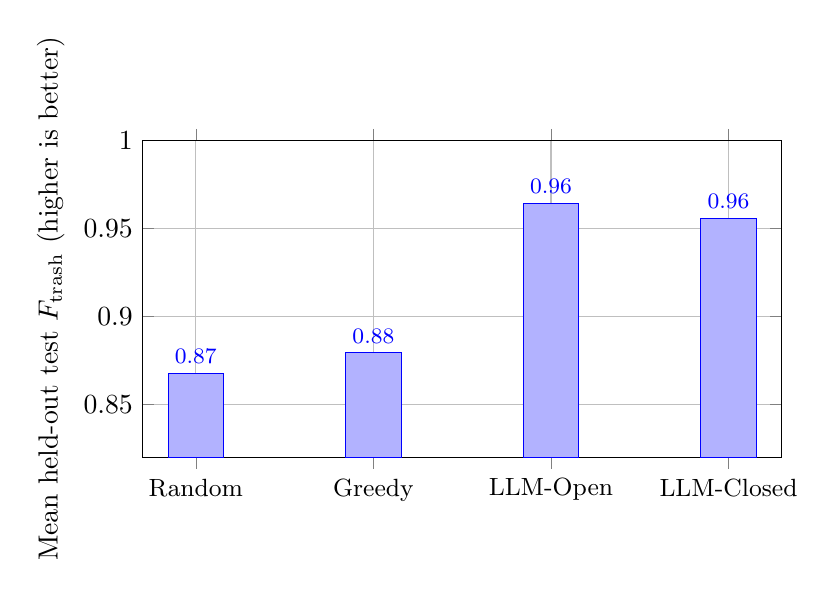
\begin{tikzpicture}
\begin{axis}[ybar,bar width=20pt,width=0.8\linewidth,height=5.6cm,ymin=0.82,ymax=1.0,
  ylabel={Mean held-out test $F_{\rm trash}$ (higher is better)},
  symbolic x coords={Random,Greedy,LLM-Open,LLM-Closed},xtick=data,
  x tick label style={font=\small},
  nodes near coords,nodes near coords align={vertical},every node near coord/.append style={font=\footnotesize},grid=major]
\addplot coordinates {(Random,0.8677) (Greedy,0.8793) (LLM-Open,0.9643) (LLM-Closed,0.9558)};
\end{axis}
\end{tikzpicture}
\caption{v4 mean held-out test trash fidelity across 12 paired seeds (seed-level distributions and bootstrap 95\% CIs are in the committed figure artifacts). All four methods search the identical neutral space with identical capacity, trainer, and budget.}
\label{fig:qae-selected}
\end{figure}

\paragraph{Paired statistics.}
All comparisons are paired per seed; $p$-values are exact two-sided Wilcoxon signed-rank tests, intervals are bootstrap 95\% CIs of the mean paired gain, and $d_z$ is Cohen's paired effect size.
\begin{itemize}[nosep]
\item LLM-Open $-$ Random: $+0.0965$ $[0.0824, 0.1120]$, $d_z=3.51$, 12/12 wins, $p=0.00049$.
\item LLM-Closed $-$ Random: $+0.0880$ $[0.0737, 0.1039]$, $d_z=3.10$, 12/12 wins, $p=0.00049$.
\item LLM-Open $-$ Greedy: $+0.0850$ $[0.0664, 0.1030]$, $d_z=2.52$, 12/12 wins, $p=0.00049$.
\item Greedy $-$ Random: $+0.0115$ $[-0.0131, +0.0347]$, $d_z=0.26$, 7/12 wins, $p=0.42$ --- parity; the v3 deficit is gone.
\item LLM-Closed $-$ LLM-Open: $-0.0085$ $[-0.0177, -0.0007]$, $d_z=-0.55$, 4/12 wins, $p=0.13$ --- no significant difference detected.
\end{itemize}

\paragraph{Refinement gains (pre-declared).}
Did the four adaptive evaluations add value over the best of the four warm starts?
For Greedy: $+0.0635$ on held-out test (95\% CI $[+0.0179, +0.1276]$), 10/12 seeds improved, Wilcoxon $p=0.0093$ --- after adequate exploration, validation-guided local refinement genuinely helps, confirming that v3 Greedy's failure was an exploration problem rather than a refinement problem.
For LLM-Closed: $+0.0185$ (95\% CI $[+0.0053, +0.0341]$), 5/12 improved and 7/12 unchanged --- a small positive contribution that does not close the gap to the open-loop batch.

\paragraph{Anytime behaviour.}
Figure~\ref{fig:qae-anytime} shows the held-out test fidelity of the best-so-far validation-selected candidate as the budget is consumed.
The LLM-Open batch is strong from its first proposal; LLM-Closed climbs through both phases; Random and Greedy track each other through the warm phase, after which Greedy's refinement pulls slightly ahead.

\begin{figure}[ht]
\centering
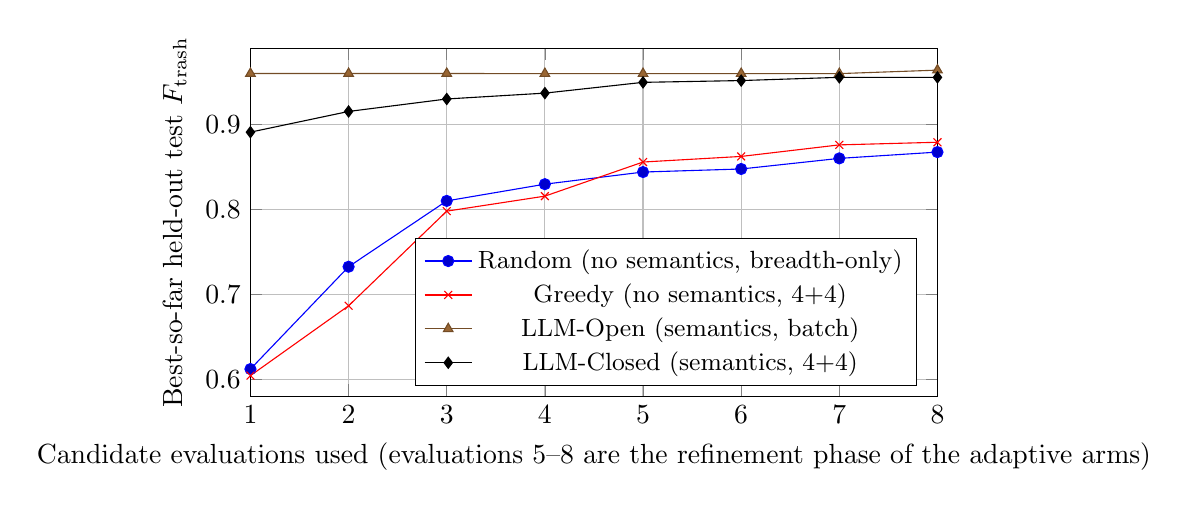
\begin{tikzpicture}
\begin{axis}[width=0.85\linewidth,height=6.0cm,xlabel={Candidate evaluations used (evaluations 5--8 are the refinement phase of the adaptive arms)},
  ylabel={Best-so-far held-out test $F_{\rm trash}$},
  xmin=1,xmax=8,ymin=0.58,ymax=0.99,xtick={1,2,3,4,5,6,7,8},grid=major,legend pos=south east,
  legend style={font=\small}]
\addplot+[mark=*] coordinates {(1,0.6120)(2,0.7326)(3,0.8102)(4,0.8299)(5,0.8442)(6,0.8478)(7,0.8603)(8,0.8677)};
\addlegendentry{Random (no semantics, breadth-only)}
\addplot+[mark=x] coordinates {(1,0.6043)(2,0.6866)(3,0.7981)(4,0.8158)(5,0.8560)(6,0.8626)(7,0.8762)(8,0.8793)};
\addlegendentry{Greedy (no semantics, 4+4)}
\addplot+[mark=triangle*] coordinates {(1,0.9603)(2,0.9603)(3,0.9603)(4,0.9602)(5,0.9602)(6,0.9602)(7,0.9602)(8,0.9643)};
\addlegendentry{LLM-Open (semantics, batch)}
\addplot+[mark=diamond*] coordinates {(1,0.8912)(2,0.9156)(3,0.9303)(4,0.9372)(5,0.9499)(6,0.9520)(7,0.9558)(8,0.9558)};
\addlegendentry{LLM-Closed (semantics, 4+4)}
\end{axis}
\end{tikzpicture}
\caption{v4 anytime performance (mean over 12 seeds; higher is better).}
\label{fig:qae-anytime}
\end{figure}

\paragraph{Proposal quality and diversity.}
Fallback accounting: Random 0/96, Greedy 0/96, LLM-Open 0/96 (its pool of eight arrived valid and distinct in one call), LLM-Closed 8/96 (5 duplicates, 3 invalid) --- down from 26/96 in v3: the diverse warm-start batch largely removed the duplicate-proposal failure mode.
Mean pairwise structural distance (fraction of differing gate slots): LLM-Closed warm batch 0.832, refinement proposals 0.658; LLM-Open first four 0.708, last four 0.615.

\paragraph{Consistency across versions.}
The semantic advantage replicates across independently drawn pools (v3 pool $0.9653$, v4 pool $0.9643$) and across spaces (rigid-layout v2: $0.9700$ against different baselines).
Random's level in the neutral space ($0.87$) is well below its rigid-space level ($0.92$): the harder the space is to search blindly, the larger the semantic-prior gain.

\section{Why the New Result Differs from the Earlier Random-Search Result}

The result does not imply that the old benchmark was wrong.
The two experiments ask different questions.

In the earlier gate-search setting, the methods largely differed in how they traversed a shared syntactic grammar.
Once capacity was controlled, the good regions of that small space were common enough that random, evolutionary, and greedy methods became practically equivalent.

In the QAE task, the prompt exposes three pieces of information that have direct architectural consequences:
\begin{enumerate}[nosep]
\item \textbf{Real state family:} RY rotations provide a natural real-amplitude parameterization.
\item \textbf{Local Hamiltonian:} the Ising chain identifies which qubits are directly correlated.
\item \textbf{Latent/trash roles:} the objective supplies a direction for information flow and disentangling.
\end{enumerate}
Ordinary random search does not condition its proposal distribution on these facts, and greedy hill-climbing conditions only on scores of its own past candidates.
The v2 RY-only control showed that the first fact alone does not explain the gap; the v3/v4 sequence shows that validation-guided adaptivity alone does not either --- with a fair multi-start allocation, Greedy reaches only Random-parity, an order of magnitude below the semantic gain.
What remains is the semantic route: converting stated physics into axis, wiring, and ordering choices before any circuit is trained.

\section{Limitations and Threats to Validity}

The present result is deliberately narrow.
It is a noiseless four-qubit statevector simulation with a single Hamiltonian family.
The API replay uses a single pinned model (\texttt{gpt-5.4-mini-2026-03-17}); a multi-model confirmatory protocol has not yet been run, so no claim attaches to any particular model family.
The prompt itself encodes hand-chosen physical hints (real amplitudes, locality, information routing); the benchmark therefore measures whether a language model can \emph{exploit} stated structure, not whether it can \emph{discover} unstated structure.
Stronger QAS methods and tensor-network-inspired baselines remain to be added.
The Greedy findings are budget-regime statements: v3 showed that a single-start allocation cannot compete with independent sampling at $B=8$, and v4 shows that four starts restore parity; larger budgets or population-based variants could behave differently again.
Because the methods differ in allocation policy as well as information content, none of the pairwise comparisons isolates a single ingredient causally.
All twelve verification replicates share the same held-out test grid, although they use independently sampled training and validation states.
Finally, while the protocol is deterministic given a machine, floating-point training is platform-dependent (third-decimal shifts across machines); all v3/v4 comparisons were computed on a single machine with identical paired seeds.

We therefore do not claim general LLM superiority, quantum advantage, or hardware relevance.
The supported claim is conditional:
\emph{when the task description exposes useful physical structure, a task-aware language-model proposal distribution can be substantially more sample-efficient than equal-capacity random architecture sampling.}

\section{Next Experiments}

A publication-quality confirmatory study should:
\begin{enumerate}
\item run a prompt-semantic ablation: the identical resource contract with the physics sentences removed, isolating the semantic content of the prompt from its formatting;
\item replay the frozen prompt across \emph{several} version-pinned LLM APIs (the present work pins one model and stores complete prompts, raw outputs, token counts, latency, and budget accounting);
\item add gradient-based QAS, restart/population variants of Greedy, and tree-tensor-network baselines;
\item probe larger budgets $B$, where local search and closed-loop feedback may matter more than at $B=8$;
\item scale to six and eight qubits and vary the latent dimension;
\item repeat on Heisenberg and molecular ground-state families;
\item add realistic noise and hardware connectivity, reporting performance--cost Pareto fronts;
\item freeze a multi-model, multi-seed confirmatory protocol before protected-test inspection.
\end{enumerate}

\section{Conclusion}

Capacity-controlled VQC benchmarks taught a negative but useful lesson: a powerful proposer cannot display meaningful reasoning if the experimental interface offers little meaningful information to reason about.
Quantum autoencoding provides a cleaner test.
By exposing the Hamiltonian, the correlation graph, and the latent/trash split while holding circuit capacity and numerical optimization fixed, the benchmark turns architecture search into a semantic design problem.
Across the single-start diagnostic (v3) and the pre-registered multi-start follow-up (v4), the picture is consistent: a version-pinned language-model proposer beats equal-budget Random in 12/12 paired seeds with or without feedback; adequate initial exploration is what makes non-semantic adaptive search competitive at all (Greedy: significantly below Random with one start, parity with four, with a genuine refinement gain); and adaptive closed-loop search shows no detectable benefit over an open-loop semantic batch at this budget.
The results separate three ingredients --- semantic proposal quality, initial exploration, and adaptive refinement --- and should be viewed as evidence for a \emph{conditional semantic-prior hypothesis}, not as a universal ranking of search algorithms.

\appendix
\section{Exact LLM prompt}
\label{app:prompt}

\paragraph{System instruction.}
\begin{quote}
You are a quantum-autoencoder circuit architect. Your job is architecture proposal, not numerical optimization. Respect the exact resource budget. Use the physical structure in the task description to propose circuit hypotheses. Return circuit structure only.
\end{quote}

\paragraph{Task instruction (v3/v4).}
\begin{quote}
Compress ground states of the 4-qubit open-chain transverse-field Ising Hamiltonian
$H=-\sum Z_iZ_{i+1}-h\sum X_i$, $h\in[0.2,2.0]$, into latent qubits $q_0,q_1$ while trash qubits $q_2,q_3$ should end in $\lvert00\rangle$.
The Hamiltonian is real in the computational basis, so its ground-state amplitudes can be chosen real.
Interactions are nearest-neighbor on the open chain $q_0$--$q_1$--$q_2$--$q_3$, so nearest-neighbor correlations are important.
Resource contract (exact, non-negotiable): the encoder is an ordered sequence of exactly 16 gates --- exactly 12 single-qubit rotations, each RX, RY, or RZ on any qubit (no per-axis quota), and exactly 4 CNOTs, each with any control and any different target (the same pair may repeat at different positions).
You choose the gate ORDER freely.
You do not choose rotation angles: a shared numerical optimizer trains all 12 angles identically for every method.
[Open loop only:] Output 8 distinct candidates.
Prefer hypotheses that (1) preserve a real-valued representation when useful and (2) route correlations/information from the trash qubits toward the latent qubits.
\end{quote}

\paragraph{JSON schema card (v3).}
\begin{quote}\small
Return ONLY a single JSON object, no prose and no markdown fences, with this schema:\\
\texttt{\{"candidates": [\{"name": "<short-id>", "gates": [}\\
\texttt{\ \ \{"g": "RY", "q": 0\}, \{"g": "CNOT", "c": 3, "t": 2\}, ...]\}]\}}\\
Each gates list holds exactly 16 entries in execution order: a rotation is \texttt{\{"g": "RX"|"RY"|"RZ", "q": 0-3\}} and a CNOT is \texttt{\{"g": "CNOT", "c": 0-3, "t": 0-3, c != t\}}. Exactly 12 rotations and exactly 4 CNOTs per candidate.
\end{quote}
If returned candidates violate the capacity contract, up to two bounded repair calls quote the rejected entries and errors and request replacements (pre-registered amendment); only then are remaining slots filled by flagged random draws.
The v4 LLM-Closed warm start uses the same task instruction with ``Output 4 distinct candidates. Aim for structural DIVERSITY across the candidates (different orderings, wirings, and axis patterns), \ldots'' in place of the open-loop closing lines.
The v1/v2 pilot used the same physics sentences with a rigid layered layout and a per-layer axes schema; that version is preserved in the repository history and \texttt{docs/research/LLM\_QAE\_SKILL.md}.

\paragraph{Closed-loop feedback template.}
After each candidate of a seed is trained, the next call appends, per earlier candidate:
\begin{quote}\small
candidate \texttt{<canonical JSON>} validation trash fidelity: \texttt{<value>} duplicate: \texttt{<true/false>}\\
Propose ONE new candidate with exactly one clearly stated structural hypothesis in its name. Do not repeat an already-evaluated candidate. Do not use or request test-set information.
\end{quote}
Protected-test values never appear in any prompt.
Up to two JSON-repair retries are allowed per call; every attempt (prompt, raw response, tokens, latency, model snapshot) is stored under \texttt{outputs/qae\_tfim\_neutral\_v3/llm\_calls/} (v3) and \texttt{outputs/qae\_tfim\_api\_v2/llm\_calls/} (v2).

\printbibliography
\end{document}
